\section{Passing Metadata Between Nodes}
To implement the ``Tainting Dependencies'' method it is necessary to pass
metadata upwards when parsing the syntax tree, such as
iterator dependencies and flags to indicate singleton nodes (for simplifications). Additionally, the
operator tree which is being built bottom-up (as described earlier in section
\ref{sect:impl:construct_mql}) is also required to be passed upwards. 

This is achieved through the \texttt{TaverseReturn}, which models a return type
when visiting nodes in the syntax tree. That is, the visitor methods are
responsible of 1) visiting any child nodes, and 2) returning an instance of the
\texttt{TraverseReturn} class based on what was returned from the child nodes,
if anything.

\subsection{The TraverseReturn Class}
The class diagram for the \texttt{TraverseReturn} class is shown in figure
\ref{fig:impl:meta:traverse_uml}. Note the flag to indicate if the current
context is a singleton, the reference to an MQL operator tree (which is being
built bottom-up), and a reference to a set of iterator dependencies (in the implementation called
\texttt{varRefs}).

\begin{figure}[!htp]
\begin{center}
  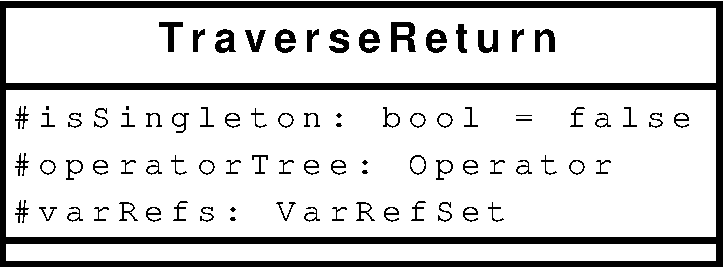
\includegraphics[scale=0.5]{diagrams/traversereturn_uml}
  \caption{TraverseReturn class diagram}
  \label{fig:impl:meta:traverse_uml}
\end{center}
\end{figure}

The \texttt{TraverseReturn} class is, as mentioned, used in the visitor when
visiting nodes in the abstract syntax tree (see section
\ref{sect:impl:context_sens_visitor}). A typical use case is shown in figure
\ref{fig:impl:meta:traverse_usage_ex}, which is an excerpt from the
implementation.

\subsection{Iterator Dependencies}
Iterator dependencies, described in section \ref{sect:trans:TD:basics}, are
passed upwards together with the MQL operator tree being built during the syntax
tree parsing process. These sets of dependencies are handled by th \texttt{VarRef} and \texttt{VarRefSet} classes.
A class diagram for these classes is shown in figure \ref{fig:impl:meta:varrefset_uml}.

\begin{figure}[!htp]
\begin{center}
  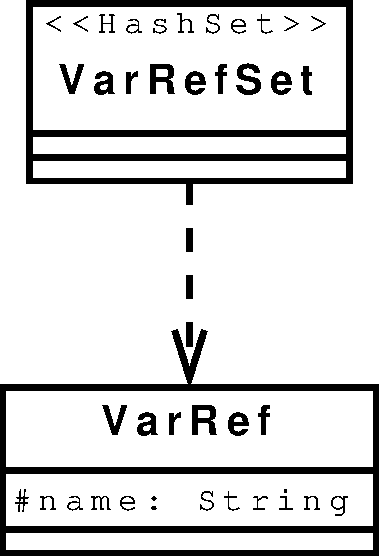
\includegraphics[scale=0.5]{diagrams/varrefset_uml}
  \caption{\texttt{VarRefSet} and \texttt{VarRef} class diagram}
  \label{fig:impl:meta:varrefset_uml}
\end{center}
\end{figure}

As described in section \ref{sect:trans:TD:dependency}, an iterator variable reference is allways dependent on
its corresponding iterator. Thus, when a iterator variable is encountered during the parse process, and the
variable is being ``read'' and not assigned or declared, the corresponding iterator is added to the current set of
iterator dependencies. The example in figure \ref{fig:impl:meta:var_ref_ex} shows the variable \texttt{\$a}
being read, in which case the iterator is added to the \texttt{TraverseReturn} to be returned's set of
dependencies.

\begin{figure}[!htp]
\begin{center}
\begin{minipage}[h]{5cm}
\begin{verbatim}
for $i in (1,2,3) return 
    ($a,4,5)
\end{verbatim}
\end{minipage}
  \caption{Example of the variable \texttt{\$a} being read. Note that the iterator
  variable \texttt{\$i} is never read}
  \label{fig:impl:meta:var_ref_ex}
\end{center}
\end{figure}

The source code excerpt in figure \ref{fig:impl:meta:var_ref_impl2} shows how
iterator dependencies are treated in the visitor implementation.

\begin{figure}[!htp]
\begin{center}
\begin{Verbatim}
// Fetch entry from symtab
SymTabEntry entry = Scope.get(tree.getChild(0).getText());
            
// Obtain and append new var ref
TraverseReturn tr = entry.getTraverseReturn();
tr.getVarRefs().add(new VarRef(tree.getChild(0).getText()));

return tr;
\end{Verbatim}
  \caption{Appending a new variable reference}
  \label{fig:impl:meta:var_ref_impl2}
\end{center}
\end{figure}

\subsection{Singleton nodes}
Singleton nodes are nodes corresponding to expressions that return a sequence of exactly one item. In
the cases where this is known to be true, the result from a translation can be
tagged with this information and used later to simplify the translation of
sequence construction (as described in section \ref{sect:impl:td:seq}).

This is the case of integer literal nodes as well as iterator variable lookups in the
symbol table. The case of integer literal nodes is shown in figure
\ref{fig:impl:meta:traverse_usage_ex} in the next section. The case of variable
lookups is somewhat counter-intuitive, since the singleton flag is actually
stored when a variable is first set. That is, the right-hand side of the
assignment is translated once and annotated with the singleton flag, which is
then set for all subsequent lookups in the symbol table. The excerpt in figure 
\ref{fig:impl:meta:var_assign_ex} shows how this is done in the implementation.

\begin{figure}[!htp]
\begin{center}
\begin{Verbatim}
// Visit children on the right side of the assignment
TraverseReturn tr = acceptThis(tree.getChild(1));

// Required for tainting deps method
Project project = new Project("[" + varName + "numb, value]", 
                      tr.getOperatorTree());

// Assign metadata
tr.setOperatorTree(project);
tr.setSingleton(true);

// Enter into symbol table
SymTabEntry tmp = Scope.set(tree.getChild(0).getText(), 
                      tr, isIterationVar);
\end{Verbatim}
  \caption[Iterator variable annontion with singleton flag]{Iterator variable
  assignment example, annotated with the singleton flag before being entered into the symtab}
  \label{fig:impl:meta:var_assign_ex}
\end{center}
\end{figure}

\subsection{Example of usage}
In the example in figure \ref{fig:impl:meta:traverse_usage_ex}, an
integer literal node is visited (a node that simply holds an integer). A
\texttt{make()} MQL operator as well as a new \texttt{TraverseReturn}
instance is created. The \texttt{make()} operator is then appended to the 
\texttt{TraverseReturn} instance, and the \textit{isSingleton} flag is set to 
\textit{true} since the result of this translation is a single item.

\begin{figure}[!htp]
\begin{center}
\begin{Verbatim}
public TraverseReturn visitIntegerLiteral(XQFTTree tree) {

    Make make = new Make("name:=[index, value], [1, " + tree.getText());
    TraverseReturn tr = new TraverseReturn();        
    tr.setSingleton(true);
    tr.setOperatorTree(make);
    return tr;
}
\end{Verbatim}
  \caption{TraverseReturn usage example}
  \label{fig:impl:meta:traverse_usage_ex}
\end{center}
\end{figure}